{
\newcommand{\Klen}{2 cm}
\newcommand{\sqth}{1.73205080757}
\newcommand{\BZ}{
	% Draw the old BZ
	\draw[BZold]
		(  0:\Klen) --
		( 60:\Klen) --
		(120:\Klen) -- 
		(180:\Klen) -- 
		(240:\Klen) -- 
		(300:\Klen) -- 
		(  0:\Klen);

	% Draw the new BZ
	\draw[BZnew]
		( 30:\Klen/\sqth) --
		( 90:\Klen/\sqth) --
		(150:\Klen/\sqth) -- 
		(210:\Klen/\sqth) -- 
		(270:\Klen/\sqth) -- 
		(330:\Klen/\sqth) -- 
		( 30:\Klen/\sqth);
}
\newcommand{\elemone}[2]
{
	\draw[fill=#1!30,draw=#1!90,rotate=#2] (0,0) -- (-30:\Klen/\sqth) -- (30:\Klen/\sqth) --cycle;
	\draw[fill=#1!30,draw=#1!90,rotate=#2,xshift=-\Klen] (0,0) -- (-30:\Klen/\sqth) -- (30:\Klen/\sqth) --cycle;
}

\newcommand{\elemtwo}[3]
{
	\draw[fill=#1!30,draw=#1!90,xscale=#3,rotate=#2]  (0,0) -- (\Klen/2,0) -- (30:\Klen/\sqth) --cycle;
	\draw[fill=#1!30,draw=#1!90,xscale=#3,rotate=#2,shift={(60:-\Klen)}] (0,0) -- (\Klen/2,0) -- (30:\Klen/\sqth) --cycle;
}

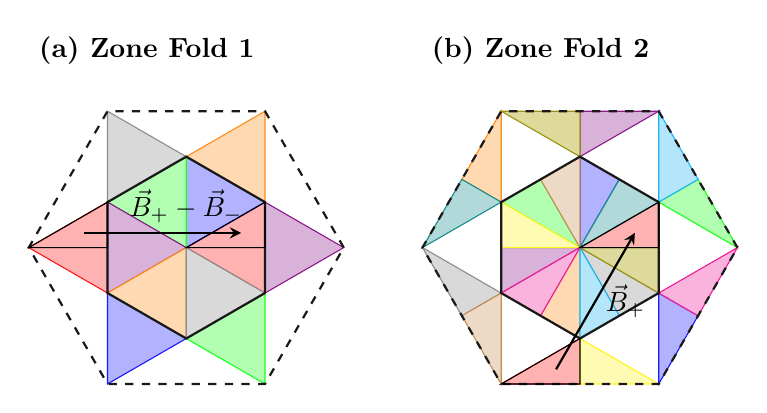
\begin{tikzpicture}[scale=1,
		BZnew/.style={color=black!90,thick},
		BZold/.style={color=black!90,thick,dashed},
		Bar/.style={color=black,thick,<-,>=stealth},
		circ2/.style={radius=1.5pt}]

	% Zone fold 1
	\begin{scope}[xshift=-2.5cm]

		% Draws the zones folding in
		\foreach \i/\colora in {0/{red},60/{blue},120/{green},180/{violet},240/{orange},300/{gray}} {
			\elemone{\colora}{\i}
		}

		% Draws on the old and new BZ
		\BZ

		% Draws the reduced symetric elemtn
		\draw[black] (0,0) -- (\Klen/2,0) -- (30:\Klen/\sqth) --cycle;
		\draw[black,xshift=-\Klen] (0,0) -- (\Klen/2,0) -- (30:\Klen/\sqth) --cycle;
		
		% Draws the arrow showing the shift in the reduced element
		\draw[Bar] (15:\Klen/\sqth/2*1.25) --node[above,xshift=.3cm]{$\vec{B}_+-\vec{B}_-$} ++(-\Klen,0);
	\end{scope}

	% Zone fold 2
	\begin{scope}[xshift=+2.5cm]

		% Draws the zones folding in
		\foreach \i/\colora in {0/{red},60/{blue},120/{green},180/{violet},240/{orange},300/{gray}} {
			\elemtwo{\colora}{\i}{1}
		}
		\foreach \i/\colora in {0/{yellow},60/{brown},120/{teal},180/{olive},240/{cyan},300/{magenta}} {
			\elemtwo{\colora}{\i}{-1}
		}

		% Draws on the old and new BZ
		\BZ

		% Draws the reduced symetric elemtn
		\draw[black] (0,0) -- (\Klen/2,0) -- (30:\Klen/\sqth) --cycle;
		\draw[black,shift={(60:-\Klen)}] (0,0) -- (\Klen/2,0) -- (30:\Klen/\sqth) --cycle;
		
		% Draws the arrow showing the shift in the reduced element
		\draw[Bar] ( 15:\Klen/\sqth/2*1.25) -- node[right]{$\vec{B}_+$} ++(240:\Klen);
	\end{scope}

	\node at (-3cm,2.5cm) {\textbf{(a) Zone Fold 1}};
	\node at (2cm,2.5cm) {\textbf{(b) Zone Fold 2}};
\end{tikzpicture}
}